% Prof. Dr. Ausberto S. Castro Vera
% UENF - CCT - LCMAT - Curso de Ci\^{e}ncia da Computa\c{c}\~{a}o
% Campos, RJ,  2022
% Disciplina: An\'{a}lise e Projeto de Sistemas
% Aluno:

\chapterimage{projeto.png} % Table of contents heading image
\chapter{Projeto do Sistema}
No capítulo a seguir serão apresentados os tipos de estratégias para construção do projeto de gerenciamento de veículos autônomos.
Será apresentado o modelo de negócio junto com os seus sub tópicos, os diagramas, arquiteturas, projeto de interface.

\section{Estrat\'{e}gia do Projeto}
Nesta seção será apresentado a estratégia de projeto juntamente com a descrição de cada proposta.
De modo a esclarecer e especificar o que é buscado ao projetar o sistema.
\subsection{Exclusividade}
O projeto é criado exclusivamente para a empresa atender suas necessidades no mercado nacional. É um modelo recomendável para grandes projetos, devido ao número de requisitos, o valor para sua implementação e os requisitos que o sistema exige, impossibilitando encontrar soluções prontas para atender aos requisitos. É um sistema que dá aos desenvolvedores mais liberdade na resolução de problemas de negócios na gestão de veículos.

Devido ao grande número de requisitos e à complexidade do sistema geral, o sistema de gerenciamento do veículo é configurado com base no modelo de sistema específico do cliente.



\subsection{Software desenvolvido}
O sistema que atende a todos os requisitos será desenvolvido pela empresa, pois seus veículos necessitam de um sistema para operá-los que não exija alteração dos requisitos do sistema. Este modelo é recomendado para empresas que não possuem necessidades específicas de negócios. Assim é possível exemplificar os seguintes sistemas: aplicativo, sistema de pagamento e controle de veículos disponíveis no sistema.

\subsection{Terceirização}
O desenvolvimento e manutenção dos veículos são realizados por outra empresa especializada na construção de veículos autónomos, é uma empresa para a manutenção dos mesmos. Este modelo é certo de saber o que a empresa está tentando alcançar, então a empresa comissionada precisa de algum conhecimento dos requisitos da empresa e necessidades de negócios.



\section{Refinamento dos Diagramas DFD e E-R}


\section{Arquitetura do Sistema - Estilos}




\subsection{Arquitetura do Sistema}

\begin{itemize}

\item \textbf{Gerenciamento}
\end{itemize}
\begin{figure}[H]
          \begin{center}
              \caption{Diagrama do sistema de dados do gerenciamento de manutenção} \label{afp}
              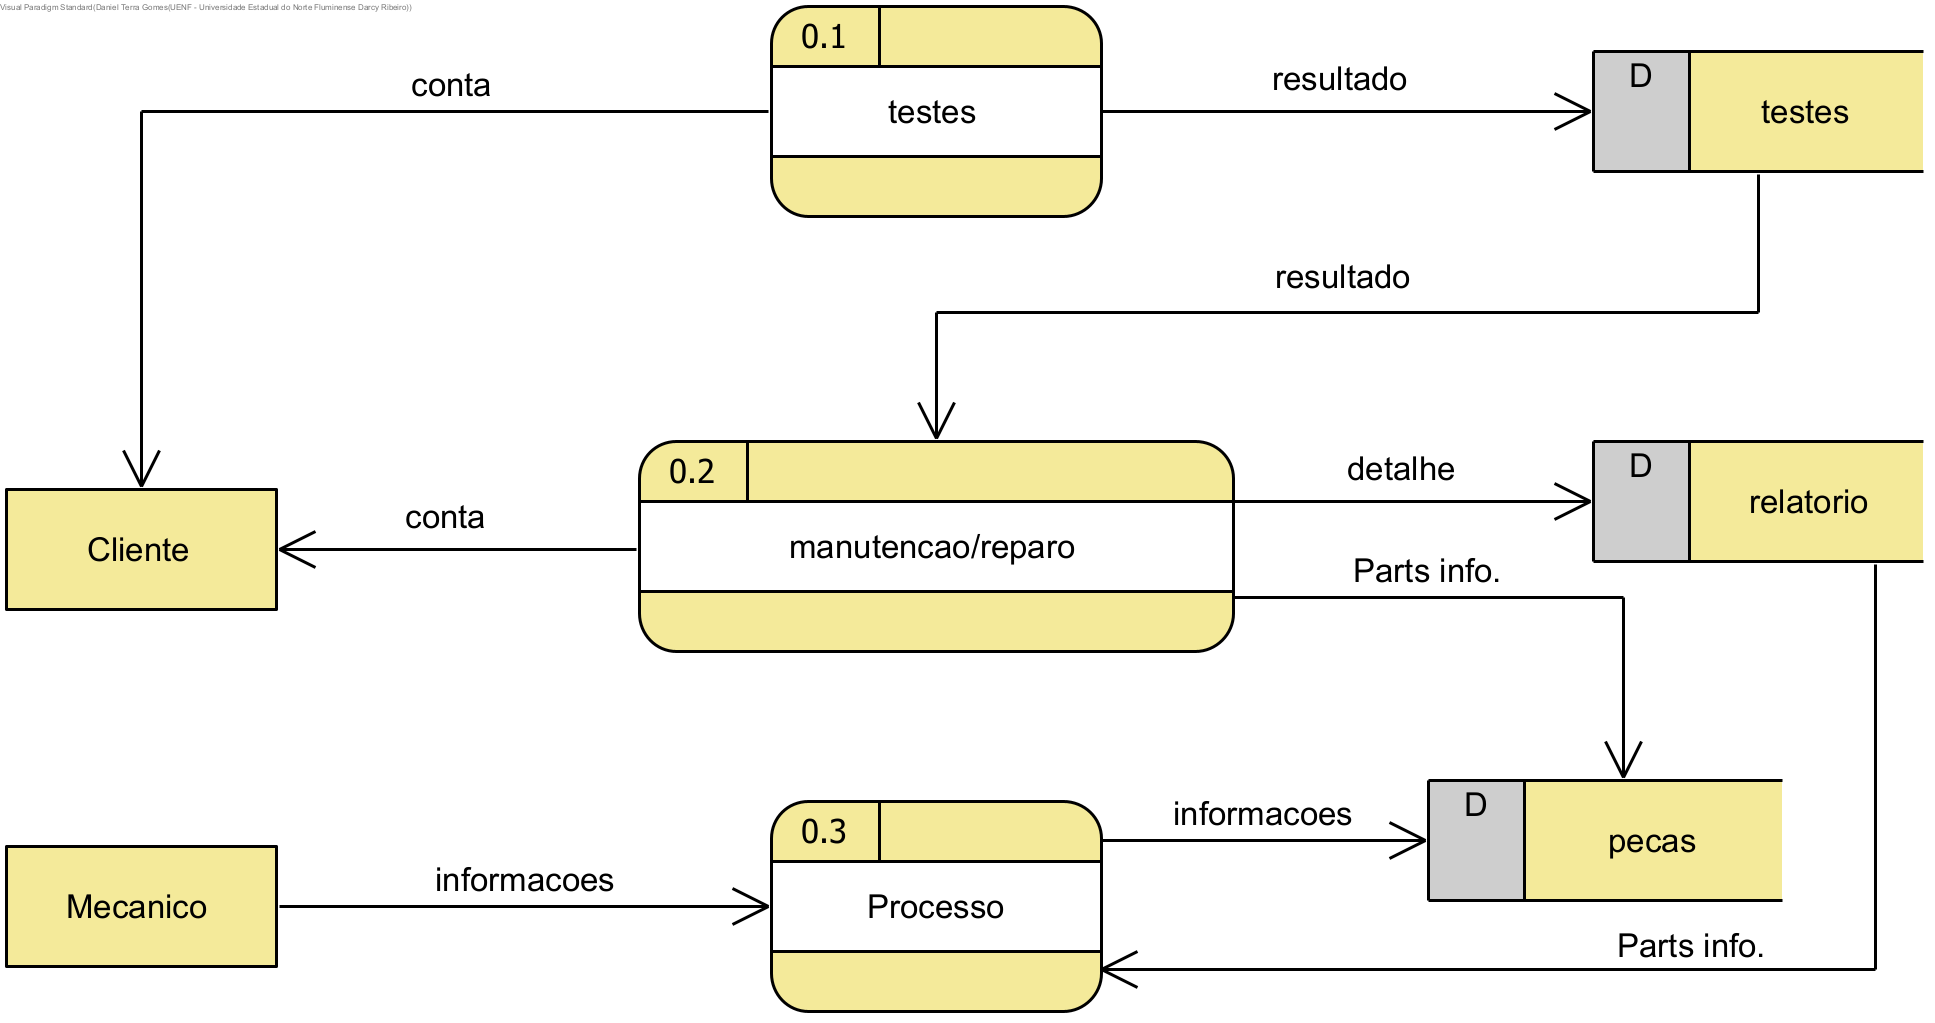
\includegraphics[width=15cm]{Depot.png} \\

          \end{center}
         \end{figure}





\subsection{Arquitetura do Hardware}


\begin{itemize}

\item \textbf{Internet}
\end{itemize}
\begin{figure}[H]
     \begin{center}
         \caption{Diagrama de internet para os atendentes} \label{afp}
         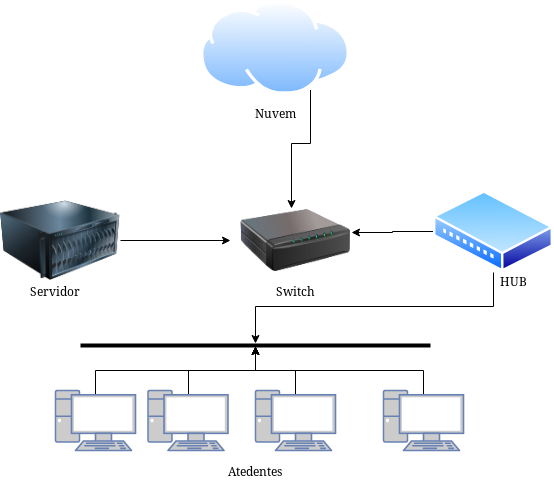
\includegraphics[width=15cm]{Pipe.png} \\

     \end{center}
    \end{figure}




\subsection{Arquitetura de Software}


\section{Projeto de Interface}
